%設定頁面
\documentclass[12pt,a4paper]{article}
\usepackage[margin=1in,a4paper]{geometry}

%設定中文
\usepackage{xeCJK} 
\setCJKmainfont{標楷體} 
\XeTeXlinebreaklocale "zh"   
\XeTeXlinebreakskip = 0pt plus 1pt 

%浮水印
%\usepackage{draftwatermark}
%\SetWatermarkText{\bf NTNU MATH}
%\SetWatermarkScale{0.7}

%圖片
\usepackage{graphicx}
\usepackage{subfigure}

%超連結
\usepackage[colorlinks,linkcolor=blue]{hyperref}

%頁首頁尾
\makeatother
\usepackage{fancyhdr}

%顏色
\usepackage{xcolor}

%表格顏色
\usepackage{colortbl}

%設定數學
\usepackage{amsmath, amsthm, amssymb}
\makeatletter

%自定圈圈標號
\usepackage{pstricks,pstricks-add}
\newcommand\textc[1]{{\begin{pspicture*}
(-0.25,-0.2)(0.25,0.3)\rput[c](0,0)
{\large \textcircled{\footnotesize #1}}
\end{pspicture*} }}

%自訂向量符號
\def\leftharpoonfill@{\arrowfill@\leftharpoonup\relbar\relbar}
\def\rightharpoonfill@{\arrowfill@\relbar\relbar\rightharpoonup}
\newcommand\rbjt{\mathpalette{\overarrow@\rightharpoonfill@}}
\newcommand\lbjt{\mathpalette{\overarrow@\leftharpoonfill@}}

%自訂定理
\newtheorem*{thm}{Theorem}
\newtheorem*{lem}{Lemma}
\newtheorem*{de}{Definition}
\newtheorem*{rmk}{Remark}
\newtheorem*{ex}{Example}
\newtheorem*{pf}{Proof}
\newtheorem*{sol}{Solution}

%程式碼
\usepackage{listings}
\usepackage{color}

\definecolor{dkgreen}{rgb}{0,0.6,0}
\definecolor{gray}{rgb}{0.5,0.5,0.5}
\definecolor{mauve}{rgb}{0.58,0,0.82}

\lstset{
  basicstyle={\small \ttfamily},
  frame=tb,
  language=Python,
  aboveskip=3mm,
  belowskip=3mm,
  showstringspaces=false,
  columns=flexible,
  basicstyle={\small\ttfamily},
  numbers=left,
  numbersep = 14pt,
  numberstyle=\tiny\color{gray},
  keywordstyle=\color{blue},
  commentstyle=\color{dkgreen},
  stringstyle=\color{mauve},
  breaklines=true,
  breakatwhitespace=true,
  tabsize=3,
  backgroundcolor=\color{gray!10}
}




%作者
\title{NTNU影像處理HW4}
\author{廖家緯}
\date{2020.4.8}

\begin{document}
\maketitle
%標題、作者、日期
\fontsize{12pt}{20pt}\selectfont
%設定字體大小、間距
\setlength{\baselineskip}{20pt}
%設定行距

\pagestyle{fancy}
\lhead{}
\chead{}
\rhead{}
\lfoot{}
\cfoot{\thepage}
\rfoot{}
\renewcommand{\headrulewidth}{0pt} %上線寬
\renewcommand{\footrulewidth}{0pt} %下線寬
%\renewcommand{\abstractname}{Executive Summary}




%正文開始
\begin{enumerate}
\item[•]{\bf Outline}:
\begin{enumerate}
\item[1.]
Develop a histogram equalization (HE) program;
\item[2.]
Apply the HE to i) gray, ii) color images;
\item[3.]
For each input image, print out the input/output images and their histograms.
\item[4.]
Discuss your experiments.
\item[•]Note that\\
For a color image $C$, 
\begin{enumerate}
\item[(i)]Convert it into a gray image $G$;
\item[(ii)]Apply HE to $G$ to get $G’$;
\item[(iii)]
For each pixel of $C$, modify its color $(r,g,b)$ by
$(r’,g’,b’) = (r,g,b) \times G’ / G$.\\
\end{enumerate}

\end{enumerate}


\item[•]
{\bf Code(Python):}
\begin{lstlisting}
# coding: utf-8

#套件
import numpy as np
import matplotlib.pyplot as plt
import cv2

# 顯示圖片
def imgshow(img):
    cv2.imshow('My Image', img)
    cv2.waitKey(0)
    cv2.destroyAllWindows()


# Histogram Equalization
def HE(img):
    [img_his, img_bin] = np.histogram(img.flatten(), range(257))
    img_cdf = np.cumsum(img_his) 
    img_m_cdf = np.ma.masked_equal(img_cdf, 0)  #除去直方圖中的0值
    img_cdf_tr = (img_m_cdf - img_m_cdf.min())*255 / (img_m_cdf.max()-img_m_cdf.min())
    img_rv = np.ma.filled(img_cdf_tr, 0).astype('uint8')  #補回0
    img_HE = img_rv[img]
    [img_HE_his, img_HE_bin] = np.histogram(img_HE.flatten(), range(257))

    #長條圖
    plt.subplot(3, 1 ,1)  #1列2行,編號1
    plt.bar(range(256), img_his, color = 'lightblue')  #原始圖片長條圖
    plt.title('Original image')
    
    plt.subplot(3, 1 ,3)  #1列2行,編號2
    plt.bar(range(256), img_HE_his, color = 'red')  #圖片HE後長條圖
    plt.title("HE's image")
    
    return img_HE


# 讀取圖檔
img = cv2.imread('image.jpg')
n = np.shape(img)[0]  #列
m = np.shape(img)[1]  #行

# 轉為灰階
gray = cv2.cvtColor(img, cv2.COLOR_BGR2GRAY)

# 灰階HE
gray_HE = HE(gray)
imgshow(gray_HE)

# 彩圖HE:分別對R,G,B做HE
[R, G, B] = cv2.split(img)
HE_R = HE(R)
HE_G = HE(G)
HE_B = HE(B)
img_HE = cv2.merge([HE_R, HE_G, HE_B])
imgshow(img_HE)

# 彩圖HE:老師給的公式
img = np.double(img)
[R, G, B] = cv2.split(img)
R_HE = R*gray_HE/gray
G_HE = G*gray_HE/gray
B_HE = B*gray_HE/gray
img_HE_tr = np.uint8(cv2.merge([R_HE, G_HE, B_HE]))
imgshow(img_HE_tr)


\end{lstlisting}

\newpage
\item[•]
{\bf Result:}
\begin{figure}[h]
\hspace*{5em}
\begin{tabular}{cc}
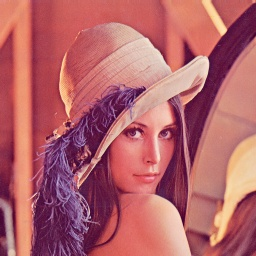
\includegraphics[height=2in]{input_image.jpg}&
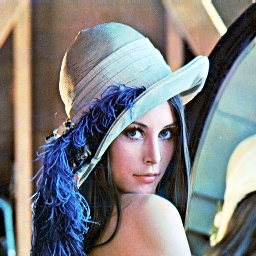
\includegraphics[height=2in]{input_image_HE.jpg}\\
彩圖  & 彩圖 Histogram Equalization \vspace*{1em}\\
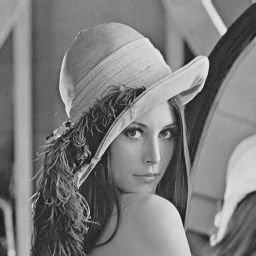
\includegraphics[height=2in]{gray_image.jpg}&
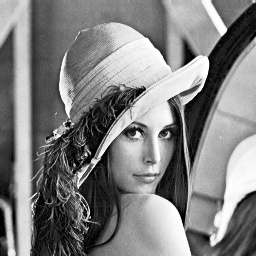
\includegraphics[height=2in]{gray_image_HE.jpg}\\
灰階  & 灰階 Histogram Equalization\\
\end{tabular}
\end{figure} 



\item[•]
{\bf Histogram:}
\begin{enumerate}

\item 灰階
\begin{figure}[h]
\hspace*{9em}
\begin{tabular}{c}
\includegraphics[height=2.2in]{gray_HE.jpg}
\end{tabular}
\end{figure}

\newpage
\item 彩圖$R$
\begin{figure}[h]
\hspace*{9em}
\begin{tabular}{c}
\includegraphics[height=2.2in]{HE_R.jpg}
\end{tabular}
\end{figure}

\item 彩圖$G$
\begin{figure}[h]
\hspace*{9em}
\begin{tabular}{c}
\includegraphics[height=2.2in]{HE_G.jpg}
\end{tabular}
\end{figure}

\item 彩圖$B$
\begin{figure}[h]
\hspace*{9em}
\begin{tabular}{c}
\includegraphics[height=2.2in]{HE_B.jpg}
\end{tabular}
\end{figure}
\end{enumerate}

\newpage
\item[•]
{\bf Experience:}\\
這次作業花了兩天的時間研究,尤其在弄懂HE的原理,過程中我不斷優化自己程式碼,也使用PIL內建函式(ImageOps.equalize)與自己的結果進行比較。另外我有用長條圖繪製每張圖片的分布,我們可以明顯發現經過Histogram Equalization後的分布更加均衡,範圍也變得比較廣,與老師PPT上的範例相同。最後感謝助教半夜的回信,讓我在崩潰的一整天後,幫助我了解PPT最後一段到底要我們做什麼。如果助教想看jupyter notebook版本可以到我的
\href{https://nbviewer.jupyter.org/github/Jia-wei-liao/Mywork/blob/master/%E5%BD%B1%E5%83%8F%E8%99%95%E7%90%86/HW4/%E5%BB%96%E5%AE%B6%E7%B7%AF.HW4.ipynb}{GitHub (點此連結) }上觀看 。
\end{enumerate}










\end{document}